\begin{figure}[t!]
\begin{center}
\centerline{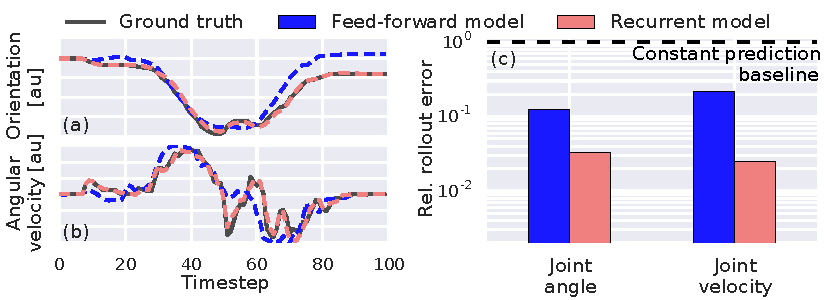
\includegraphics[width=1\columnwidth]{figures/real_jaco_rollout}}
\vspace{-0.1in}
\caption{Real and predicted test trajectories of a JACO robot arm. The recurrent model tracks the ground truth (a) orientations and (b) angular velocities closely. (c) The total 100-step rollout error was much better for the recurrent model, though the feed-forward model was still well below the constant prediction baseline. A video of a Mujoco rendering of the true and predicted trajectories: \href{\rolloutsrealjaco}{\rolloutsrealjaconame}.
}
\label{fig:real_jaco_rollout}
\end{center}
\vskip -0.25in
\end{figure}